\section{2020 年 11 月 3 日答疑记录}

\begin{example}
    指出下列函数的单调性和值域:
    \begin{twocolpro}
    (1) $f(x)=x^2+|x|-2$; & (2) $g(x)= \dfrac{3x+1}{x-1}$.
    \end{twocolpro}
\end{example}
\begin{solution}
    (1) 方法一: 根据绝对值的定义可知,
    \[f(x)=\begin{cases}
        x^2+x-2,& x\geqslant 0,\\
        x^2-x-2,& x< 0.
        \end{cases}\]
    函数的图形如下 (分别作 $y$~轴左侧和右侧的图形):
    
    \begin{center}
        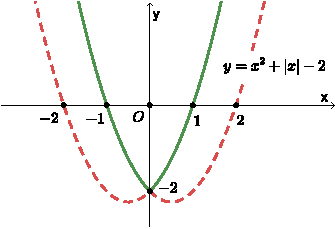
\includegraphics[scale=1.1]{2020-1126-1945-crop}
    \end{center}
    
    由图得, $f(x)$ 在 $(-\infty,0)$ 上单调递减, 在 $[0,+\infty)$ 上单调递增, 值域为 $[-2,+\infty)$.
    
    方法二: 因为 $f(-x)=f(x)$, 所以 $f(x)$ 为偶函数, 图形关于 $y$~轴对称. 令 $x\geqslant 0$ 知, $f(x)=x^2+x-2$, 可作出 $f(x)$ 在 $y$~轴右侧的图形, 再关于 $y$~轴作对称图形即可. 答案同上. 
    
    (2) 将函数变形 (把分子写成 ``分母的倍数'' 加 ``常数'' 的形式, 再拆项),
    \[g(x)= \frac{3(x-1)+4}{x-1}= 3+\frac4{x-1},\]
    由此可知, $g(x)$ 的图形可由 $h(x)=\dfrac4x$ 的图形向右平移一个单位长度, 再向上平移三个单位长度得到:
    
    \begin{center}
        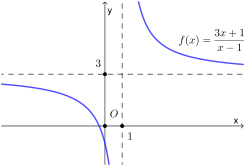
\includegraphics[scale=1]{2020-1126-2225-crop}
    \end{center}
    
    所以, $g(x)$ 在 $(-\infty,1)$ 和 $(1,+\infty)$ 上均单调递减, 值域为 $(-\infty,3)\cup (3,+\infty)$.
\end{solution}

\begin{example}
    已知 $f(2x)$ 的定义域为 $[0,1)$, 求 $f(x)$ 和 $f(x+3)$ 各自的定义域.
\end{example}
\begin{solution}
    注意, 定义域是当前函数表达式中 $x$ 的取值范围, 而同一个函数 (作用法则) 的作用范围是不会改变的.
    
    因为 $f(2x)$ 的定义域为 $[0,1)$, 此时 $x\in[0,1)$ 且 $f$ 作用在 $2x$ 上, 所以 $f$ 的作用范围为 $[0,2)$, 表明 $f(x)$ 的定义域为 $[0,2)$ (因为此时 $f$ 作用在 $x$ 上, 定义域与作用范围相同).
    
    对 $f(x+3)$, 因为 $f$ 作用在 $x+3$ 上, 所以 $x+3\in[0,2)$, 解得 $x\in[-3,-1)$, 即 $f(x+3)$ 的定义域为 $[-3,-1)$.
\end{solution}

\begin{example}
    已知 $A=\{x\mid a+1<x<2a+4\}$, $B=\{x\mid -1\leqslant x\leqslant 5\}$, 且 $A\subseteq B$ 成立, 求 $a$ 的取值范围.
\end{example}
\begin{solution}
    (1) 若 $A=\varnothing$, 则 $a+1\geqslant 2a+4$, 解得 $a\in(-\infty,-3]$.
    
    (2) 若 $A\neq\varnothing$, 则 
    \[-1\leqslant a+1< 2a+4\leqslant 5,\]
    解得 $a\in\biggl[-2,\dfrac12\biggr]$.
    
    综上所述, $a\in(-\infty,-3]\cup \biggl[-2,\dfrac12\biggr]$
\end{solution}

\begin{example}
    解不等式:
    \begin{twocolpro}
    (1) $|4-2x|>2$; & (2) $\dfrac1{x+1}\geqslant 2$.
    \end{twocolpro}
\end{example}
\begin{solution}
    (1) 绝对值的几何意义是: $|a|$ 表示数轴上点 $a$ 到原点的距离, 所以 $|4-2x|>2$ 表明
    \[4-2x<-2\quad\text{或}\quad 4-2x>2,\]
    解得 $x\in(-\infty,1)\cup (3,+\infty)$.
    
    (2) 移项通分, 化成分式与 $0$ 比, 再转化为等价的乘积与 $0$ 比:
    \[\frac1{x+1}-2\geqslant 0
        \Rightarrow \frac{-1-2x}{x+1}\geqslant 0
        \Rightarrow \left\{\!\!\begin{array}{l}
            (2x+1)(x+1)\geqslant 0,\\
            x+1\neq 0,
            \end{array}\right. \]
    解得 $x\in \biggl(-1,\dfrac12\biggr]$.
\end{solution}